\chapter{Timing: Setup, Hold and Clock Speed}
\label{ch:timing}

How fast can a chip run? What limits it? Why can one mistake be fixed by slowing the clock while another makes the chip useless at any speed? This chapter answers those questions. Timing is the single most important topic in digital hardware interviews, and it is the foundation for the clock divider, pipeline and FIFO questions later in the book.

\section{Synchronous design}

Almost every digital chip follows one pattern, called \term{synchronous design}: banks of flip-flops (registers) hold the current state, blocks of combinational logic compute the next state from it, and one shared clock tells every flip-flop to capture its new value at the same moment (Figure~\ref{fig:syncpath}).

\begin{figure}[h]
\centering
\begin{tikzpicture}
  \dbox{a}{(0,0)}{launch FF}{1}
  \draw[thick] (2.6,0.6) rectangle (5.4,2.4); \node[align=center,font=\small] at (4,1.5) {combinational\\logic};
  \dbox{b}{(6.5,0)}{capture FF}{1}
  \draw (a-q) -- (2.6,1.5); \draw (5.4,1.5) -- (b-d);
  \draw (a-d) -- ++(-0.6,0);
  \draw (b-q) -- ++(0.6,0);
  \draw (a-clk) -- ++(-0.4,0) |- (-0.4,-0.7) -- (6.1,-0.7) |- (b-clk);
  \draw (-0.4,-0.7) -- ++(-0.8,0) node[left]{$CLK$};
\end{tikzpicture}
\caption{The basic timing path: a launch flip-flop, logic, and a capture flip-flop on the same clock.}
\label{fig:syncpath}
\end{figure}

At each rising clock edge, the launch flip-flop sends out a new value. It ripples through the logic. At the \emph{next} rising edge, the capture flip-flop must grab the result. The whole chip advances one step per clock cycle, and as long as every path obeys two timing rules, gate delays never cause errors. Those two rules are the subject of this chapter.

\section{The clock}

A clock is a square wave. Its \term{period} $T$ is the time between rising edges; its \term{frequency} is $f = 1/T$. A 2\,GHz clock has a 500\,ps period. The \term{duty cycle} is the fraction of the period the clock spends high, normally 50\%.

\section{Timing parameters}

Every flip-flop and logic block has a few timing numbers:

\begin{itemize}
  \item \term{Setup time} $t_{su}$: how long \emph{before} the clock edge the input $D$ must be stable.
  \item \term{Hold time} $t_h$: how long \emph{after} the clock edge $D$ must stay stable.
  \item \term{Clock-to-Q delay} $t_{cq}$: how long after the clock edge the output $Q$ changes.
  \item For the logic: the \term{propagation delay} $t_{pd}$ (slowest path, time until the output is final) and the \term{contamination delay} $t_{cd}$ (fastest path, time until the output first starts changing), as in Chapter~\ref{ch:comb}.
\end{itemize}

\begin{figure}[h]
\centering
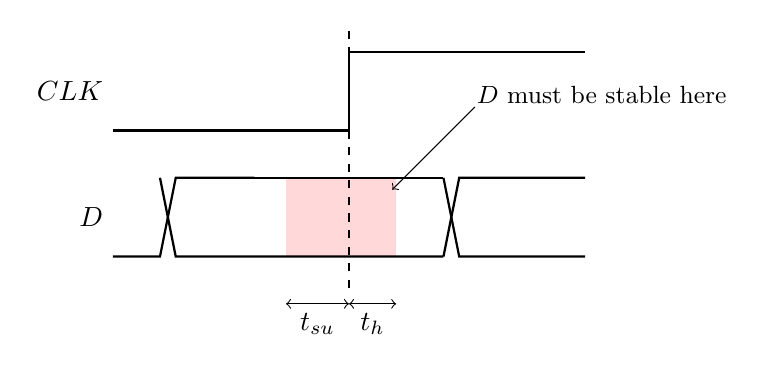
\begin{tikzpicture}[scale=1.0]
  \draw[thick] (0,2) -- (3,2) -- (3,3) -- (6,3);
  \node[left] at (0,2.5) {$CLK$};
  \fill[red!15] (2.2,0.4) rectangle (3.6,1.4);
  \draw[thick] (0,0.4) -- (0.6,0.4) -- (0.8,1.4) -- (1.8,1.4);
  \draw[thick] (1.8,1.4) -- (4.2,1.4);
  \draw[thick] (0.6,1.4) -- (0.8,0.4) -- (1.8,0.4) -- (4.2,0.4);
  \draw[thick] (4.2,0.4) -- (4.4,1.4) -- (6,1.4); \draw[thick] (4.2,1.4) -- (4.4,0.4) -- (6,0.4);
  \node[left] at (0,0.9) {$D$};
  \draw[dashed] (3,0) -- (3,3.3);
  \draw[<->] (2.2,-0.2) -- node[below]{$t_{su}$} (3,-0.2);
  \draw[<->] (3,-0.2) -- node[below]{$t_h$} (3.6,-0.2);
  \node[font=\small,anchor=west] at (4.5,2.45) {$D$ must be stable here};
  \draw[->] (4.6,2.3) -- (3.55,1.25);
\end{tikzpicture}
\caption{$D$ must not change inside the shaded window around the clock edge: from $t_{su}$ before it to $t_h$ after it.}
\label{fig:window}
\end{figure}

If $D$ changes inside that window (Figure~\ref{fig:window}), the flip-flop may capture the wrong value or go metastable (Chapter~\ref{ch:latch}).

\section{The setup constraint: how fast can the clock go?}

Follow the data launched at one clock edge (time 0) to the capture flip-flop.
\begin{enumerate}
  \item The launch flip-flop's output changes at $t_{cq}$.
  \item The change ripples through the logic and settles by $t_{cq} + t_{pd}$.
  \item The capture flip-flop samples at the next edge, time $T$, and needs the data stable $t_{su}$ before that.
\end{enumerate}
So the data must arrive in time:
\[
  \boxed{t_{cq} + t_{pd} + t_{su} \le T}
\]
The minimum period is the sum on the left, and the maximum frequency is its reciprocal:
\[
  f_{max} = \frac{1}{t_{cq} + t_{pd} + t_{su}}.
\]

\begin{bigidea}
The setup constraint is about data arriving \emph{too late}. It is set by the slowest path (the \term{critical path}), and it depends on the clock period. If it fails, you can always fix it by slowing the clock down.
\end{bigidea}

\begin{worked}{maximum clock frequency}
$t_{cq} = 50$\,ps, the slowest logic path $t_{pd} = 400$\,ps, $t_{su} = 30$\,ps.
\[
  T_{min} = 50 + 400 + 30 = 480~\text{ps}, \qquad f_{max} = \frac{1}{480~\text{ps}} \approx 2.08~\text{GHz}.
\]
\end{worked}

\begin{worked}{the logic budget}
A design must run at 500\,MHz ($T = 2$\,ns). Its flip-flops have $t_{cq} = 0.3$\,ns and $t_{su} = 0.2$\,ns. What is the longest the logic may take?
\[
  t_{pd} \le T - t_{cq} - t_{su} = 2 - 0.3 - 0.2 = 1.5~\text{ns}.
\]
\end{worked}

\section{The hold constraint: data arriving too early}

There is a second, sneakier danger. At the same clock edge at which the capture flip-flop samples the \emph{old} data, the launch flip-flop is sending \emph{new} data. If that new data races through a very short path and arrives before the capture flip-flop's hold time is over, it corrupts the value being captured.

The earliest the new data can arrive is $t_{cq} + t_{cd}$ (using the fastest clock-to-Q and the fastest logic path). It must not arrive before the hold window closes:
\[
  \boxed{t_{cq} + t_{cd} \ge t_h}
\]

\begin{bigidea}
The hold constraint involves only \emph{one} clock edge, the same edge launching and capturing, so \textbf{the clock period does not appear in it}. A hold violation cannot be fixed by slowing the clock. A chip with a hold violation fails at every frequency. It is fixed by \emph{adding delay} (buffers) to the too-fast path.
\end{bigidea}

\begin{worked}{a hold violation}
$t_{cq} = 40$\,ps, the shortest logic path is 10\,ps, $t_h = 60$\,ps.
Arrival $= 40 + 10 = 50$\,ps $< 60$\,ps: a hold violation of 10\,ps. Lowering the frequency changes nothing. Add at least 10\,ps of delay on the short path (in practice, a little more for margin).
\end{worked}

\begin{trap}
``The chip fails a timing check; can we fix it by lowering the clock frequency?'' Yes for setup, \emph{no} for hold. This is one of the most common true/false questions. A related trap: adding logic delay \emph{helps} hold and \emph{hurts} setup.
\end{trap}

\section{Clock skew and jitter}

So far we assumed the clock reaches every flip-flop at the same instant. In reality the clock travels through wires and buffers, and different flip-flops receive it at slightly different times. The difference is \term{clock skew}. Define
\[
  t_{skew} = (\text{clock arrival at capture FF}) - (\text{clock arrival at launch FF}).
\]
Positive skew means the capture flip-flop's clock arrives later.

With skew, the constraints become:
\[
  \text{setup: } t_{cq} + t_{pd} + t_{su} \le T + t_{skew}, \qquad
  \text{hold: } t_{cq} + t_{cd} \ge t_h + t_{skew}.
\]

Positive skew gives the data extra time to arrive before the capture edge, which \textbf{helps setup}. But it also keeps the capture flip-flop's hold window open later, which \textbf{hurts hold}. Negative skew does the opposite. Skew is a trade: whatever it gives one constraint, it takes from the other.

\term{Jitter} is random variation in the clock edge timing from cycle to cycle. Because nobody can predict it, it always eats into the margin; for setup, it effectively shortens the period.

\begin{worked}{skew in a clock buffer}
At 500\,MHz, $t_{cq} = 0.3$\,ns, $t_{su} = 0.2$\,ns, and the capture flip-flop's clock passes through one extra buffer of 0.1\,ns, so $t_{skew} = +0.1$\,ns. The logic budget becomes
\[
  t_{pd} \le T + t_{skew} - t_{cq} - t_{su} = 2 + 0.1 - 0.3 - 0.2 = 1.6~\text{ns}.
\]
If the hold time is 0.15\,ns, the shortest path must satisfy $0.3 + t_{cd} \ge 0.15 + 0.1$: true for any $t_{cd} \ge 0$, so hold is safe.
\end{worked}

\section{Slack}

Timing tools report \term{slack}: how much margin a path has.
\[
  \text{setup slack} = (T + t_{skew}) - (t_{cq} + t_{pd} + t_{su}), \qquad
  \text{hold slack} = (t_{cq} + t_{cd}) - (t_h + t_{skew}).
\]
Positive slack means the path passes with that much to spare; negative slack is a violation. \term{Static timing analysis} (STA) tools compute the slack of every path in a chip, using worst-case delays, without simulating any data.

\section{Reading timing diagrams}

Assessment questions often show a waveform and ask for the output. The method:
\begin{enumerate}
  \item Mark every active clock edge (usually rising).
  \item At each edge, read the value of $D$ just \emph{before} the edge (that is what is captured).
  \item Draw $Q$ changing to that value a little after the edge ($t_{cq}$), and holding until the next edge.
  \item For a chain of flip-flops, repeat stage by stage: each stage's input is the previous stage's output, which changed only just after the edge, so each stage sees the \emph{old} value at that edge.
\end{enumerate}

\begin{figure}[h]
\centering
\begin{tikztimingtable}[timing/slope=0.05, xscale=1.5, yscale=1.2]
$CLK$ & LL HH LL HH LL HH LL HH LL \\
$D$   & L HHHH LLL LLLL HHHH LL \\
$Q_1$ & 2.3L 4H 8L 3.7H \\
$Q_2$ & 6.3L 4H 7.7L \\
\extracode
\begin{pgfonlayer}{background}
\vertlines[help lines]{2,6,10,14}
\end{pgfonlayer}
\end{tikztimingtable}
\caption{Two flip-flops in a row ($D \to Q_1 \to Q_2$). Each output changes slightly after a rising edge (gridlines). $Q_2$ copies $Q_1$ one cycle later.}
\label{fig:twoflops}
\end{figure}

\section{Shift registers and hold time}

A \term{shift register} is a chain of flip-flops with each $Q$ wired directly to the next $D$, no logic in between. On each clock edge every bit moves one place along. Because there is no logic, $t_{cd} = 0$, and the hold check is simply $t_{cq} \ge t_h + t_{skew}$.

\begin{worked}{a 4-bit shift register}
Four D flip-flops form a shift register. Each has $t_{cq} = 50$\,ps (positive) and $t_h = 0$.
\begin{itemize}
  \item With zero skew: $50 \ge 0$. Hold is met. Each stage captures its neighbor's old value before the neighbor changes, and the register shifts exactly one place per edge.
  \item Now suppose the clock reaches each flip-flop 60\,ps later than the one before it ($t_{skew} = +60$\,ps along the shift direction). Hold requires $50 \ge 0 + 60$: violated. The new value from one flip-flop arrives at the next one before that one's (late) clock edge, so data can skip through two stages in one cycle and bits are lost.
  \item Fix: route the clock the other way (so skew is negative along the data direction), or add delay between stages.
\end{itemize}
\end{worked}

\begin{onoa}
A reported question describes a 4-bit shift register of D flip-flops with positive clock-to-Q delay and zero hold time. The point being tested: with no logic between stages, correct shifting depends on $t_{cq}$ being larger than the hold time plus any skew. With $t_h = 0$ and no skew, any positive $t_{cq}$ works.
\end{onoa}

\section{Pipelining}
\label{sec:pipelining}

If the critical path is too slow for the clock you want, you can split the logic into stages with registers between them. This is \term{pipelining}.

\begin{worked}{pipelining a slow block}
A 900\,ps block of logic sits between two registers whose overhead is $t_{cq} + t_{su} = 100$\,ps. The clock period must be at least 1000\,ps (1\,GHz). Split the logic into three 300\,ps stages with registers between: each stage needs $300 + 100 = 400$\,ps, so the clock can run at 2.5\,GHz.
\begin{itemize}
  \item \textbf{Throughput} (results per second) rises from 1 to 2.5 billion: a new input enters every 400\,ps.
  \item \textbf{Latency} (time for one input to come out) rises from 1000\,ps to $3 \times 400 = 1200$\,ps.
\end{itemize}
\end{worked}

Pipelining trades latency for throughput. Its returns diminish: each extra stage adds another $t_{cq} + t_{su}$ of overhead, and stages can never be perfectly balanced. Processor pipelines (Chapter~\ref{ch:arch}) are the most famous example.

\section{Long wires and retiming flip-flops}
\label{sec:retiming}

On a large chip, just sending a signal across the die can take longer than a clock period. The fix is the same idea as pipelining: insert flip-flops along the wire so that each segment fits in one cycle. These are sometimes called \term{pipeline} or \term{retiming flops}.

\begin{worked}{flip-flops on a long wire}
A signal must travel 60\,mm between two flip-flops. The wire (with repeaters) has a delay of 0.1\,ns per mm. The clock period is 5\,ns, and each flip-flop's overhead is $t_{cq} + t_{su} = 0.2$\,ns. Assume the clock arrives everywhere at the same time.

Total wire delay: $60 \times 0.1 = 6$\,ns, longer than one period. Each segment can use at most $5 - 0.2 = 4.8$\,ns, which covers $4.8/0.1 = 48$\,mm. Segments needed: $\lceil 60/48 \rceil = 2$. Two segments need \textbf{one} extra flip-flop in the middle. The signal now takes two cycles to arrive.
\end{worked}

\begin{onoa}
A reported question gives two flip-flops 60\,mm apart, data and clock wire delays, and a 5\,ns period, and asks for the minimum number of retiming flip-flops. If the clock is routed along with the data, its wire delay creates skew: add the skew to the time each segment may use (positive skew in the data direction helps setup). Then divide the total data delay by the time per segment, round up to get segments, and subtract one to get flip-flops.
\end{onoa}

\section{Time borrowing with latches}

Latch-based designs can do something flip-flop designs cannot. Because a latch is transparent for a whole clock phase, data that arrives late at a latch is not lost; it passes through while the latch is open, and the next stage simply starts late. A slow stage can \term{borrow time} from a fast one that follows it. This is one reason high-performance custom designs sometimes use latches instead of flip-flops, despite their harder timing analysis.

\section{Special paths and sign-off corners}

\begin{itemize}
  \item A \term{false path} is a path that exists in the wiring but can never actually carry a meaningful transition (for example, through two muxes whose selects are never set that way together). It is excluded from timing checks.
  \item A \term{multicycle path} is allowed more than one clock cycle by design (for example, a slow divider whose result is only read every other cycle).
  \item Timing must be met across manufacturing and operating variation (Chapter~\ref{ch:pvt}). \textbf{Setup} is checked at the \textbf{slow} corner (slow transistors, low voltage, worst temperature), where paths are longest. \textbf{Hold} is checked at the \textbf{fast} corner, where short paths are shortest.
\end{itemize}

\section{Making and distributing the clock}

\begin{itemize}
  \item A \term{phase-locked loop} (PLL) generates a fast, stable clock from a slower reference crystal, by multiplying its frequency.
  \item A \term{clock tree} distributes the clock to millions of flip-flops through a balanced network of buffers (H-trees, meshes, spines) designed to keep skew small.
  \item \term{Clock gating} turns off the clock to idle flip-flops to save power (Chapter~\ref{ch:power}). It must be done with a special cell (a latch plus an AND gate) so the gated clock never glitches.
  \item A group of flip-flops driven by one clock forms a \term{clock domain}. Signals that cross between domains need special handling (Chapter~\ref{ch:rtl}).
\end{itemize}

\section{Summary}

\begin{itemize}
  \item Setup: $t_{cq} + t_{pd} + t_{su} \le T + t_{skew}$. It limits frequency; fix it by slowing the clock, shortening logic, or pipelining.
  \item Hold: $t_{cq} + t_{cd} \ge t_h + t_{skew}$. No $T$ in it; fix it by adding delay, never by slowing the clock.
  \item Positive skew (capture clock late) helps setup and hurts hold.
  \item Slack is the margin; negative slack is a violation.
  \item In a timing diagram, each flip-flop captures the value just before the edge and changes $t_{cq}$ after it.
  \item Shift registers depend on $t_{cq} > t_h + t_{skew}$.
  \item Pipelining raises throughput and frequency but adds latency and register overhead.
  \item Long wires need retiming flip-flops: segments $= \lceil \text{wire delay} / (T - \text{overhead}) \rceil$, flops $=$ segments $- 1$.
  \item Setup is signed off at the slow corner, hold at the fast corner.
\end{itemize}

\section{Exercises}

\begin{enumerate}
  \item $t_{cq} = 80$\,ps, $t_{pd} = 600$\,ps, $t_{su} = 40$\,ps, no skew. What is the maximum clock frequency?
  \item $t_{cq} = 30$\,ps, $t_{cd} = 5$\,ps, $t_h = 50$\,ps. Is there a hold problem? How would you fix it?
  \item The capture clock arrives 40\,ps after the launch clock. Does this help or hurt setup? Hold?
  \item A design targets 1\,GHz with $t_{cq} = 100$\,ps and $t_{su} = 50$\,ps. What is the maximum logic delay?
  \item A 1200\,ps logic block with 100\,ps of register overhead is split into four equal pipeline stages. Find the new clock frequency, and compare the latency before and after.
  \item A shift register has $t_{cq} = 50$\,ps and $t_h = 20$\,ps. Does it work with zero skew? With the capture clock 40\,ps late at every stage?
  \item True or false: a hold violation can be fixed by lowering the clock frequency.
  \item At which process corner is setup timing checked? Hold timing?
  \item A 50\,mm wire has 0.08\,ns/mm delay. The clock period is 1\,ns and flip-flop overhead is 0.2\,ns. How many retiming flip-flops are needed?
  \item In Figure~\ref{fig:twoflops}, what is the value of $Q_2$ just after the third rising edge?
\end{enumerate}

\subsection*{Answers}
\begin{enumerate}
  \item $T = 80 + 600 + 40 = 720$\,ps, so $f_{max} \approx 1.39$\,GHz.
  \item Yes: $30 + 5 = 35 < 50$, a 15\,ps violation. Add at least 15\,ps of delay to the short path. Changing the frequency will not help.
  \item That is $+40$\,ps skew: it helps setup (40\,ps more time) and hurts hold (the hold requirement grows by 40\,ps).
  \item $1000 - 100 - 50 = 850$\,ps.
  \item Each stage: $300 + 100 = 400$\,ps, so 2.5\,GHz. Latency before: $1200 + 100 = 1300$\,ps. After: $4 \times 400 = 1600$\,ps.
  \item Zero skew: $50 \ge 20$, works. With $+40$\,ps skew: $50 \ge 20 + 40 = 60$ fails, a 10\,ps hold violation.
  \item False.
  \item Setup: slow corner. Hold: fast corner.
  \item Each segment may use $1 - 0.2 = 0.8$\,ns, covering 10\,mm. Total 50\,mm needs 5 segments, so 4 flip-flops.
  \item Before the third edge, $Q_1$ is 0 (it captured $D = 0$ at the second edge), so $Q_2$ becomes 0. (At the second edge $Q_2$ captured $Q_1 = 1$; at the third it captures $Q_1 = 0$.)
\end{enumerate}
